\documentclass[a4paper,12pt]{article}
\usepackage{amsmath}
\usepackage[utf8]{inputenc}  
\usepackage{graphicx}       
\usepackage{geometry}
\usepackage{parskip}
\usepackage{textcomp}
\usepackage{wrapfig}
\usepackage{caption}
\usepackage{listings}
\usepackage{xcolor}
\usepackage[inkscapelatex=false]{svg}
\usepackage[
backend=biber,
style=apa,
sorting=ynt
]{biblatex}

\addbibresource{sources.bib}


\definecolor{darkgreen}{rgb}{0.0, 0.5, 0.0}
\lstdefinelanguage{RAPID    }{
  morekeywords={MODULE, PROC, VAR, CONST, IF, THEN, ELSE, WHILE, FOR, TO, ENDFOR, RETURN, TRUE, FALSE, PERS, TASK, ENDPROC, ENDIF, ENDWHILE, TEST, CASE, DEFAULT, ENDTEST, STOP, ERROR, TRAP, CONNECT, DISCONNECT, RAISE, EXIT, ENDTRAP, WITH},
  sensitive=true,
  morecomment=[l]{!},       % Single-line comment
  morecomment=[s]{/*}{*/},   % Multi-line comment
  morestring=[b]{"}         % Strings wrapped in "
}

\lstdefinestyle{rapidstyle}{
  language=RAPID,
  basicstyle=\ttfamily\footnotesize,
  keywordstyle=\color{blue}\bfseries,
  stringstyle=\color{red},
  commentstyle=\color{darkgreen},
  numbers=left,
  numberstyle=\tiny,
  frame=single,
  backgroundcolor=\color{gray!10},
}

\lstset{style=rapidstyle}

\geometry{a4paper, margin=2.5cm} 

\begin{document}

\begin{titlepage}
    \centering
    \pagenumbering{gobble}
    \vfill
    
    \title{ABB RobotStudio, YuMi Application \& YuMi Challenge \\ \large TEL200 technical report\vspace{10cm}}
    \author{J\o rgen Asmundvaag \\ Ludvik H\o ibjerg-Aslaksen \\ Christopher Ljosland Strand}
    \date{March 2025}
    \maketitle
    \vfill
    \begin{figure}
        \includesvg[width=0.45\columnwidth]{NMBU_logo.svg}
    \end{figure}
    \vfill
\end{titlepage}

\section{Abstract}
Jørgen Asmundvaag
Ludvik Høibjerg-Aslaksen
Christopher Ljosland Strand

NMBU, February-March 2025.

This lab project consists of two problems that can be solved with the collaborative robot ABB YuMi IRB® 1400. 

YuMi Application i
The purpose of the YuMi Application is to move geometric objects to another position and back to their position. This is achieved by applying the theory on joints, poses, and kinematics for robotic arms. By developing and testing on the YuMi, we were able to achieve a looping program for moving all the geometric forms forward and back to the starting point. 

For the YuMi Challenge, we chose to create a program that enables us to play chess against the robot. This was achieved by using our knowledge gained during the YuMi Application, and developing further in RobotStudio. By the end of the project period, we got the YuMi to play the scholar's mate against a human, in a collaborative environment. With the ADD MORE HERE AND REWORD PARAGRAPHS

\pagenumbering{arabic} % nah, ikke noe sånt her. Bruk heller de gode gamle europeiske

\newpage
\tableofcontents
\newpage

\section{Introduction}
Industrial robotics plays an increasingly vital role in modern manufacturing, increasing productivity, precision, and efficiency. ABB RobotStudio and the RAPID language provides a powerful platform for simulating and developing robotic operations in a virtual environment prior to physical implementation. This report presents two distinct tasks, each detailed in the sections below.

The first task called \textit{YuMi Application}, the goal of this task was to move three different shaped objects from their initial position to their designated final position. 

The second application is the \textit{YuMi challenge} where we were given a open-ended task to test the capabilities of the YuMi robot. Inspired by the famous 18th-century chess automaton \textit{The Mechanical Turk}\cite{mechanicalturk2025}, we decided to have to YuMi Robot play chess against us. Like \textit{The Mechanical Turk} the YuMi Robot is not autonomous and it uses pre-programmed moves to execute the Scholar's Mate. This  will provide an understanding of the functionality of YuMi robot and it´s capabilities doing precise tasks.

\section{Method}
\subsection{Theory}
In this chapter, some important concepts are presented to help understand how a robotic arm moves.

\subsubsection{Poses}
The pose of an object describes its position and orientation relative to a known reference point. It can be mathematically represented using a homogeneous transformation matrix:

\[
T = 
\begin{bmatrix}
R & t \\
0 & 1
\end{bmatrix}
\]

- \( R \) represents orientation (rotation matrix).
\\
- \( t \) represents position (translation vector).

\[
\begin{array}{c@{\hspace{2cm}}c}
\text{2D:} &
\text{3D:} \\
\begin{bmatrix}
r_{11} & r_{12} & x \\
r_{21} & r_{22} & y \\
0 & 0 & 1
\end{bmatrix}
&
\begin{bmatrix}
r_{11} & r_{12} & r_{13} & x \\
r_{21} & r_{22} & r_{23} & y \\
r_{31} & r_{32} & r_{33} & z \\
0 & 0 & 0 & 1
\end{bmatrix}
\end{array}
\]


\subsubsection{Path and Trajectory}
A \textit{path} defines how the robot moves from one pose to another, without specifying timing. A \textit{trajectory} includes timing information, determining how fast and when the robot passes through each point along the path.

\subsubsection{Joint space and Cartesian space}
Robot motion can be calculated in either \textit{joint space} or \textit{Cartesian space}:

- \textbf{Joint space} represents the robot's configuration using joint angles. It allows for simpler calculations but typically results in curved paths for the end-effector, which may be unsuitable for tasks requiring straight-line precision \parencite{corke2017}.

- \textbf{Cartesian space} plans motion based on the end-effector's position in space, enabling accurate, linear movements. However, it involves more complex computations and can lead to high joint velocities, especially near singularities—poses where the robot's movement becomes limited.

\subsubsection{Singularities}
Singularities are specific configurations where the robot loses some freedom of movement. This can cause instability or high joint speeds. Robots with more joints, like YuMi, can avoid these situation because of the 7 joints and therefore more suitable for more versatile tasks. 

\subsection{YuMi Application}
The workstation contains a cube, cylinder, and prism, each with two slots arranged in a 3x3 grid. The task is to move the objects between slot 1 and 3 and return to the start upon button press. No changes to the object models were needed, as they were already implemented.

\subsubsection{Creating the Paths and Targets}
The grid is defined from the global coordinate system, with 100 mm between each slot center. Columns represent slot positions (x-axis), and rows define object types (y-axis). The robot moves each object from column 1 to 3 or vice versa.

Since the gripper aligns its local coordinate system with the object's, all target frames must be rotated 180° around the x- or y-axis. For the cube, we define an approach point above and a grasp point below to avoid collisions. The cylinder follows a similar setup but requires precise centering. The prism requires an additional 90° rotation to allow gripping it by its corner and side for a secure hold.

\subsubsection{Code Structure and Timings}
At the top of the RAPID code, all targets are defined along with two key variables: \textit{speed} and \textit{precision}, controlling motion timing and accuracy.

The main logic is inside a \texttt{while} loop that continuously checks button inputs. Depending on the button pressed and direction, the code calls specific functions to move the corresponding object accordingly.

\iffalse
For example, when the green button with the signal \textit{di\_cube} is pressed, the program first determines the direction the cube should move, subsequently calling either the \textit{cube\_left\_right} or \textit{cube\_right\_left} functions. These functions guide the robot to an upper target point, open the gripper, move down to grasp the object, close the gripper, move back up, transfer to the opposite side, descend again, release the object, and finally return to the starting position. The same logic and procedure is similar for the cylinder and prism.
\fi

When the green button \textit{di\_cube} is activated, the program evaluates the cube’s current position and calls either \textit{cube\_left\_right} or \textit{cube\_right\_left} to execute the appropriate path. Each function moves the robot to a predefined approach point, opens the gripper, descends to the grasping position, closes the gripper, lifts the object, transfers it to the target slot, lowers it, releases the object, and returns to the home position. The same control logic is applied to both the cylinder and prism, with minor variations for geometry handling.

\subsubsection{Creating The Mechanism Of The Emergency Button}
\iffalse
\begin{wrapfigure}{r}{0.25\textwidth}
  \label{fig:create_joint}
  \centering
  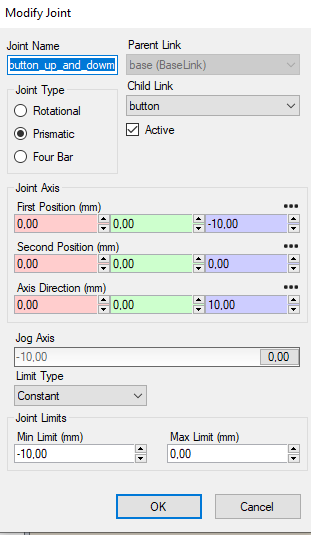
\includegraphics[width=0.2\textwidth]{create_joint.png}
  \caption{Create joint}
\end{wrapfigure}
\fi
The first step towards animating the button is to create a mechanism. This can be done by pressing the create mechanism button under the modeling tab.

The second step is to create links and joints. First create the links with the e-stob base as the baselink, and the e-stop button as childlink. Then to create joints choose prismatic as the joint type.

The button travels along the z-axis in the negative direction therefore the min limit is set to -10 mm and max limit to 0 mm. After this has been done the mechanism is done and compile mechanism can be pressed. The final step is to make a pressed pose such that it can be moved with smart components.

\subsubsection{Simulating The Emergency Button}
The emergency stop button needs to stop all movements when pressed and when let go, start all movement. To achieve this a trap routine must be used, this due it's ability to interrupt a command at any moment. The trap routine can be created using the syntax below:
\begin{lstlisting}
    TRAP EmergencyStop
        StopMove;
        WaitUntil di_EmergencySituation = 0;
        StartMove;
    ENDTRAP
\end{lstlisting}
This trap routine when called stops all movement then waits until the emergency button no longer is pressed. Under module a interrupt number needs to be defined this allows the program to use a interrupt in the code. This can be done by writing: 
\begin{lstlisting}
VAR intnum stop_emer; ! interrupt number datatype
\end{lstlisting}
After this the interrupt number stop\_emer needs to be connected to a trap routine. Using the CONNECT keyword can achieve this it also needs to be defined as the correct interrupt signal type this can be doing by using ISignalDI. All of this needs to be written under main.
\begin{lstlisting}
    ! Connects the intnum with the trap routine EmergencyStop
    CONNECT stop_emer WITH EmergencyStop;
    ! Handles checking wether the emergency stop button is pressed
    ISignalDI di_EmergencySituation, high, stop_emer;
\end{lstlisting}

When a pose mover receives a high signal to its Execute it will move the mechanism to that pose. Using a NOT gate the Execute on a pose mover can be set to high when the input is low such the unpressed state is active when input is low. The input is connected directly to pose mover for the pressed state so the pose mover will be in its pressed pose when the input is high. The input is also connect to directly to the output for use later in station logic. See figure~\ref{fig:smart_component_emer} for a picture of the smart component.
\begin{center}
    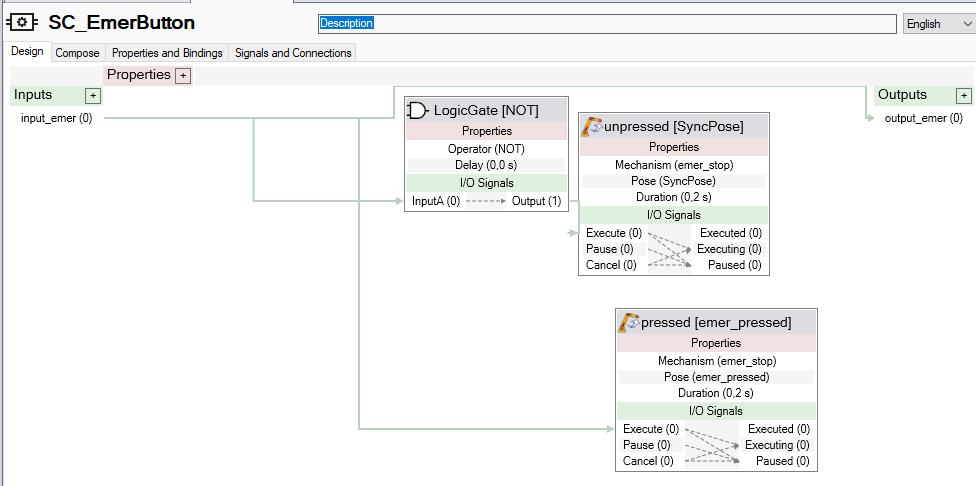
\includegraphics[width=0.8\linewidth]{SC_emer_button.png}
    \captionof{figure}{Smart component of the emergency button}
    \label{fig:smart_component_emer}
\end{center}
To connect the functionality of the emergency button to the simulated movement a few connections in station logic is required. First connect do\_EmergencySituation to input of the emergency button smart component then connect the output of the emergency button smart component to di\_EmergencySituation. When do\_EmergencySituation is set to high the button will move and execute the trap routine.

\subsection{YuMi Challenge}
\subsubsection{CAD geometry}
To be able to get accurate placements of the chess pieces, we modeled a chessboard using the Rectangle surface geometry option in RobotStudio. Using this we created a 25x25mm square surface, and assembled a chessboard from 64 of these rectangles. We centered the board axis to align with the target of the wobj0, to simplify our setup process. We also aligned the border of the board 200 mm from the wobj0 target. We created targets for the center of each chess board square, to place the pieces correctly. 

To create the CAD geometry, we used a 3D-scanner borrowed from Eiklab to make a 3D object for each type of chess piece. Then imported each 3D file into Fusion360 where we performed the following steps:
\begin{enumerate}
    \item Mesh $\rightarrow$ Insert $\rightarrow$ Insert Mesh
    \item Rotated the chess pieces such that they are straight
    \item Exported them as .sat files
\end{enumerate}
When all .sat files were finished we imported the them into Robotstudio using the import CAD geometry button. After importing the pieces we positioned them at their correct places using trial and error, and then used duplicate to get a piece at every spot.

\subsubsection{Creating the paths and targets}
\label{sec:Challenge_paths_targets}
When creating the paths, we based the targets on the chess moves from table~\ref{tab:chess_moves}.

\begin{table}[h] %Scholar's mate moves
    \centering
    \begin{tabular}{c l l}
        \hline
        Move & White & Black \\
        \hline
        1. & e4 & e5 \\
        2. & Dh5 & Sc6 \\
        3. & Lc4 & Sf6?? \\
        4. & Dxf7 & (checkmate) \\
        \hline
    \end{tabular}
    \caption{Scholar's Mate}
    \label{tab:chess_moves}
\end{table}
To make the YuMi Robot's moves as smooth as possible it is important to have two targets above the desired destination. One that is about 5 mm above the chess piece and one that is higher in the range 25-50 mm above the piece. This allows the YuMi Robot to move smoothly between each target. Due to the 3D-scans being somewhat inaccurate the distances specified before may need some adustments depending on the piece and quality of the model.

To simplify the paths the YuMi Robot returns to a set point after picking up or placing a piece. This point is centered above the queen with a 25 mm offset towards the YuMi Robot. 

After the paths have been created it is important to note that a fully extended gripper would collide with pieces surrounding the piece to be picked up. To solve this the RAPID command \textit{g\_MoveTo value;} was used. This command extends the gripper to the specified value allowing the gripper to easily slide between the pieces. The space between chess pieces is about 7 mm for the large pieces and about 8 mm for pawns.

After finishing moving all the chess pieces, the YuMi robot moves its arm in a celebration like movement. When running the celebration the arm has to move quite far up, so to achieve this a helping point has to be used to avoid collisions.

\subsubsection{Code structure and timings}
The top part located within the module part consist of all the targets and three variables called speed, precision and timing. The variables control how fast the YuMi Robot moves, how precise and seconds between each  chess move. The main body of the RAPID code consists of while loop that is constantly true allowing the code to run in a loop, within the while loop the code has several if statements that check whether the buttons have been pressed or not. 

The green button \textit{di\_cube} when pressed runs move 1 from table~\ref{tab:chess_moves}. When it is pressed a second time it runs move 2 and so on. After all moves are run it resets to move 1. The second blue button \textit{di\_cylinder} runs all moves with timing delay specified in the code by a variable. The third red button \textit{di\_prism} runs the celebration described in section \ref{sec:Challenge_paths_targets}. The fourth yellow button \textit{di\_home} returns the YuMi Robot to its start position.

The final button is an emergency stop button called \textit{di\_EmergencySituation} this button when pressed runs a trap routine that stops the YuMi Robot mid path, and when let go it continues the operation. One of the main perks to using a trap routine is that it can interrupt any movement and then issue a command which the it would not be able to do with if statements.

\subsubsection{Physical development}
To get a chess board with the same size as the one from the simulation, we had to create a custom board. This was done using Figma where we created an A4 frame with 25x25mm squares, and a cross marking the center in each square. This then got exported as a PDF and was printed out. 
\section{Results}
\subsection{YuMi Application}
For the YuMi Application task, we found several results during our work on the robot. By applying the knowledge on poses and joints from the lectures, we managed to move all the geometric forms both to the other side, and back to their starting position. 


In the first versions of our code, we encountered several errors with the robot moving in the wrong direction, or having an error in joint limits. This proved as challenging to solve, but 



\subsubsection{Challenges}
The greatest challenge we faced during our work on the YuMi Application, was in regards to poses and singularities. 
The YuMi has 7 degrees of freedom and is a redundant manipulator.

\subsection{YuMi Challenge}
For the YuMi Challenge, we managed to play the Scholar's mate against a person, using the collaborative 
\subsubsection{Challenges}

After achieving a working simulation, we tested it on the actual robot, but encountered issues not present in the simulation. Movements that functioned well in simulation caused collisions or exceeded joint limits in practice. To address this, intermediate help points can be added to guide the robot safely around obstacles. However, the primary issue usually arises from inconsistent axis configurations across target points, causing unexpected rotations or joint over extensions. Ensuring consistent axis configurations for all points within the same path effectively resolves this problem.

\subsection{YuMi Challenge}
The YuMi challenge did not present significant issues regarding configurations; however, we encountered challenges related to the precision required when playing chess with a robotic arm. Specifically, ensuring that the arm or gripper avoided accidental contact with other pieces while grabbing or placing chess pieces demanded careful attention. To resolve this, we adjusted the height of the arm movements to prevent unwanted contact. During placement, problems arose from either missing the intended target or unintentionally knocking over adjacent pieces, largely because such conditions weren't visible in simulations. Introducing helping points or raising the pieces slightly mitigated these difficulties.
Additionally, we encountered an issue where the gripper had sticky tape on it, causing pieces to become stuck during handling. 
After these issues were tackled it worked flawlessly and the celebration added at the end also worked as intended.

\section{Discussion}
\subsection{YuMi Application}
\subsubsection{Paths}

One area we could have improved, would be on the paths that the robot are following. We have seen improvements in every version of our program, and we feel that the paths that ended up being in the program are the simplest and most linear we have managed to create. But there are definitely an area of improvement, especially for clearance. Even though the robot is moving clear of any objects and collisions, we are aware of some positions on the path where the arm could benefit from more distance from both the table and the robot body.

\subsection{YuMi Challenge}
\subsubsection{Expansion}
For the YuMi Challenge, we decided to hard code the moves of the common schools´ mate. Although we think this is sufficient to show of the YuMi´s application in a collaborative environment in regard to the time at hand, we see the possibility to expand its moves and game playing ability. 

One area we could have improved, would be on the paths that the robot are following. We have seen improvements in every version of our program, and we feel that the paths that ended up being in the program are the simplest and most linear we have managed to create. But there are definetily an area of improvement, especially for clearance. Even though the robot is moving clear of any objects and collisions, we are aware of some positions on the path where the arm could benefit from more distance from both the table and the robot body.

\subsection{YuMi Challenge}
\subsubsection{Expansion}
For the YuMi Challenge, we decided to hard code the moves of the common schools´ mate. Although we think this is sufficient to show of the YuMi´s application in a collaborative environment in regard to the time at hand, we see the possibility to expand its moves and gameplaying ability. 

Before deciding on defining the moves as paths, we explored the possibility of using the buttons as forward/backward, left/right and pick up/down buttons. This would emulate a game controller, making it possible to play all possible moves.  


Before deciding on defining the moves as paths, we explored the possibility of using the buttons as forward/backward, left/right and pick up/down buttons. This would emulate a game controller, making it possible to play all possible moves.  

\section{Conclusions} 
The ABB YuMi 1400 cobot is powerful and versatile. During the projects we have seen both its capabilities and its limitations. 
having the opportunity  to develop in RobotStudio, test our code on the robot, debug and go back to RobotStudio abled us to quickly patch bugs, test new approaches and refine our code. 

For the YuMi Challenge, having the freedom to choose our task, gave us another view on working with cobots, and 

During this project we have tested and seen both the possibilities and limits of the current state of the art of collaborative robots. With the YuMi application we were able to practice and learn the basics of RobotStudio and developing with RAPID
\nocite{*} % outputs everything without them being cited in the text
\printbibliography
\end{document}